\chapter{Conversion Service}

\section{Methodology}

The objective of the Conversion Service is to convert a given set of input WHIs into dzi files. Since a dzi is layered into a pyramid scheme, it is necessary to calculate the needed number of levels, as well as the dimensions of each level (see fig. 3.1 for an example).

\begin{figure}[H]
	\begin{center}
		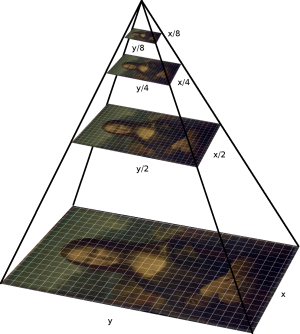
\includegraphics[scale=0.5]{img/pyramid.png}
		\caption{Example of a pyramid scheme in image processing (source: http://iipimage.sourceforge.net/images/pyramid.png)}
		\label{fig:fig3.1}
	\end{center}
\end{figure}

Therefore, the Conversion Service must be able to open an WHI $img_{input}$ of any of the in 2.2.1 defined formats. Based on the size of $img_{input}$ the number of necessary levels $lvl$ must be calculated. Once $lvl$ has been determined, $img_{input}$ must be resized into an appropriate scale for each $lvl_i$ in $lvl$. The resized image will be called $img_i$, with $i$ representing the corresponding level. In the next step, every $img_i$ will be tessellated into $x*y$ tiles. Each tile will be referrenced via $t^i_{r,c}$, with $r$ being the row and $c$ being the column of the tile in $whi_i$. To complete the conversion, the Conversion Service must create a describing xml file for each converted image $img_{dzi}$.


\subsection{Creating a Deep Zoom Image}
\subsection{Deepzoom.py}
% ways to create dzi
% why deepzoom.py
% who does it work

\section{Implementation}
\section{Test}
\subsection{Setup}
\subsection{Result}